\documentclass{practice}

\usepackage[dvipsnames]{xcolor}

\title{4}
\date{\DTMdate{2024-10-02}}

\usetikzlibrary{positioning,calc}

\usepackage{listings}

\begin{document}
\maketitle

\begin{task}{Modes and questions and modes and questions and \dots}
  For each of the modes of operation seen in class explain the following:
  \begin{itemize}
    \item how decryption works,
    \item what happens with the plaintext after a bit flip in a ciphertext block,
    \item whether random reads are possible and why,
    \item whether encryption and decryption can be done in parallel and why,
    \item if the mode of operation resembles a stream cipher,
    \item if so, is it a synchronous or self-synchronising stream cipher.
  \end{itemize}
\end{task}

\begin{task}{Security expectations}
  Explain why randomised encryption is important for confidentiality.
  Is confidentiality all we need for secure data exchange?
\end{task}

\begin{task}{The ShiftRows cipher}
  Recall that the AES \texttt{ShiftRows} algorithm is given by

  \begin{figure}[h!]
    \centering
    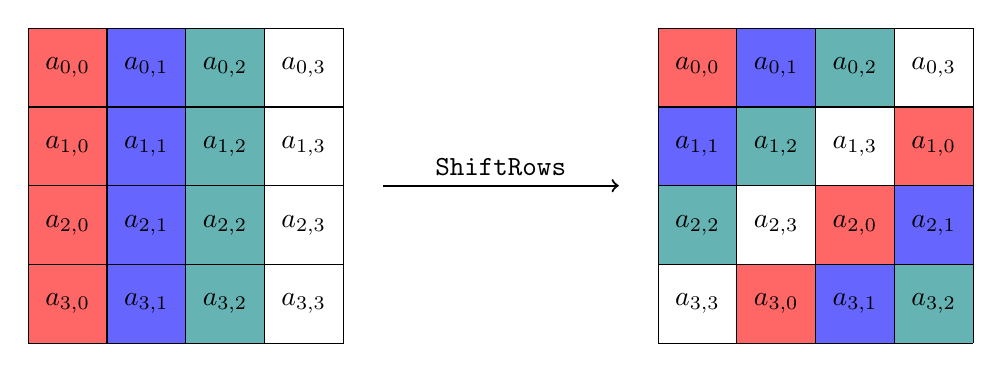
\begin{tikzpicture}
      \begin{scope}

        \fill[red,opacity=0.6] (0,3) rectangle ++ (1,1) node[black,opacity=1,pos=.5] {$a_{0,0}$};
        \fill[red,opacity=0.6] (0,0) rectangle ++ (1,1) node[black,opacity=1,pos=.5] {$a_{3,0}$};
        \fill[red,opacity=0.6] (0,1) rectangle ++ (1,1) node[black,opacity=1,pos=.5] {$a_{2,0}$};
        \fill[red,opacity=0.6] (0,2) rectangle ++ (1,1) node[black,opacity=1,pos=.5] {$a_{1,0}$};
  
        \fill[blue,opacity=0.6] (1,3) rectangle ++ (1,1) node[black,opacity=1,pos=.5] {$a_{0,1}$};
        \fill[blue,opacity=0.6] (1,0) rectangle ++ (1,1) node[black,opacity=1,pos=.5] {$a_{3,1}$};
        \fill[blue,opacity=0.6] (1,1) rectangle ++ (1,1) node[black,opacity=1,pos=.5] {$a_{2,1}$};
        \fill[blue,opacity=0.6] (1,2) rectangle ++ (1,1) node[black,opacity=1,pos=.5] {$a_{1,1}$};
      
        \fill[teal,opacity=0.6] (2,3) rectangle ++ (1,1) node[black,opacity=1,pos=.5] {$a_{0,2}$};
        \fill[teal,opacity=0.6] (2,0) rectangle ++ (1,1) node[black,opacity=1,pos=.5] {$a_{3,2}$};
        \fill[teal,opacity=0.6] (2,1) rectangle ++ (1,1) node[black,opacity=1,pos=.5] {$a_{2,2}$};
        \fill[teal,opacity=0.6] (2,2) rectangle ++ (1,1) node[black,opacity=1,pos=.5] {$a_{1,2}$};

        \draw (3,3) rectangle ++ (1,1) node[black,opacity=1,pos=.5] {$a_{0,3}$};
        \draw (3,0) rectangle ++ (1,1) node[black,opacity=1,pos=.5] {$a_{3,3}$};
        \draw (3,1) rectangle ++ (1,1) node[black,opacity=1,pos=.5] {$a_{2,3}$};
        \draw (3,2) rectangle ++ (1,1) node[black,opacity=1,pos=.5] {$a_{1,3}$};
  
        \draw (0,0) grid (4,4); 
      \end{scope}

      \draw[thick,->] (4.5,2) -- (7.5,2) node[midway,above]{\texttt{ShiftRows}};
  
      \begin{scope}[shift={(8,0)}]
        \fill[red,opacity=0.6] (0,3) rectangle ++ (1,1) node[black,opacity=1,pos=.5] {$a_{0,0}$};
        \fill[red,opacity=0.6] (1,0) rectangle ++ (1,1) node[black,opacity=1,pos=.5] {$a_{3,0}$};
        \fill[red,opacity=0.6] (2,1) rectangle ++ (1,1) node[black,opacity=1,pos=.5] {$a_{2,0}$};
        \fill[red,opacity=0.6] (3,2) rectangle ++ (1,1) node[black,opacity=1,pos=.5] {$a_{1,0}$};
  
        \fill[blue,opacity=0.6] (1,3) rectangle ++ (1,1) node[black,opacity=1,pos=.5] {$a_{0,1}$};
        \fill[blue,opacity=0.6] (2,0) rectangle ++ (1,1) node[black,opacity=1,pos=.5] {$a_{3,1}$};
        \fill[blue,opacity=0.6] (3,1) rectangle ++ (1,1) node[black,opacity=1,pos=.5] {$a_{2,1}$};
        \fill[blue,opacity=0.6] (0,2) rectangle ++ (1,1) node[black,opacity=1,pos=.5] {$a_{1,1}$};
      
        \fill[teal,opacity=0.6] (2,3) rectangle ++ (1,1) node[black,opacity=1,pos=.5] {$a_{0,2}$};
        \fill[teal,opacity=0.6] (3,0) rectangle ++ (1,1) node[black,opacity=1,pos=.5] {$a_{3,2}$};
        \fill[teal,opacity=0.6] (0,1) rectangle ++ (1,1) node[black,opacity=1,pos=.5] {$a_{2,2}$};
        \fill[teal,opacity=0.6] (1,2) rectangle ++ (1,1) node[black,opacity=1,pos=.5] {$a_{1,2}$};

        \draw (3,3) rectangle ++ (1,1) node[black,opacity=1,pos=.5] {$a_{0,3}$};
        \draw (0,0) rectangle ++ (1,1) node[black,opacity=1,pos=.5] {$a_{3,3}$};
        \draw (1,1) rectangle ++ (1,1) node[black,opacity=1,pos=.5] {$a_{2,3}$};
        \draw (2,2) rectangle ++ (1,1) node[black,opacity=1,pos=.5] {$a_{1,3}$};
  
        \draw (0,0) grid (4,4); 
      \end{scope}
    \end{tikzpicture}
    \caption{AES \texttt{ShiftRows} operation.}
  \end{figure}

  Suppose now that the \texttt{ShiftRows} operation is used as a block cipher such that:
  \begin{itemize}
    \item Two consecutive message bytes are taken at a time, and their bits are written in \emph{column-major} order into the box.
    \item The bits of the key are written in column-major order into the box and XORed with the message bits in place.
  \end{itemize}

  Encrypt the message \texttt{LYNX} with the \texttt{ShiftRows} cipher given the IV \texttt{0xECF1} and the key \texttt{0xCE67} by using the CBC mode of operation.

  \begin{table}[h!]
    \centering
    \begin{tabular}{@{}lcccccccccccccc@{}}
      Letter & A  & B  & C  & D  & E  & F  & G  & H  & I  & J  & K  & L  & M & \dots\\\midrule
      DEC & 65 & 66 & 67 & 68 & 69 & 70 & 71 & 72 & 73 & 74 & 75 & 76 & 77 & \dots\\
      HEX & 41 & 42 & 43 & 44 & 45 & 46 & 47 & 48 & 49 & 4A & 4B & 4C & 4D & \dots\\\\
      Letter & \dots & N  & O  & P  & Q  & R  & S  & T  & U  & V  & W  & X  & Y  & Z\\\midrule
      DEC & \dots & 78 & 79 & 80 & 81 & 82 & 83 & 84 & 85 & 86 & 87 & 88 & 89 & 90\\
      HEX & \dots & 4E & 4F & 50 & 51 & 52 & 53 & 54 & 55 & 56 & 57 & 58 & 59 & 5A
    \end{tabular}
    \caption{ASCII character codes of capital English letters.}
  \end{table}
\end{task}

\begin{task}{Substitution madness}
  The AES S-box is given in \autoref{table:aessbox}, where the column is determined by the least significant nibble and the row by the most significant nibble of a byte.
  \begin{table}[h!]
    \centering
    \ttfamily
    \begin{tabular}{@{}c|cccccccccccccccc@{}}
         & 00 & 01 & 02 & 03 & 04 & 05 & 06 & 07 & 08 & 09 & 0A & 0B & 0C & 0D & 0E & 0F\\
      \midrule
      00 & 63 & 7C & 77 & 7B & F2 & 6B & 6F & C5 & 30 & 01 & 67 & 2B & FE & D7 & AB & 76\\
      10 & CA & 82 & C9 & 7D & FA & 59 & 47 & F0 & AD & D4 & A2 & AF & 9C & A4 & 72 & C0\\
      20 & B7 & FD & 93 & 26 & 36 & 3F & F7 & CC & 34 & A5 & E5 & F1 & 71 & D8 & 31 & 15\\
      30 & 04 & C7 & 23 & C3 & 18 & 96 & 05 & 9A & 07 & 12 & 80 & E2 & EB & 27 & B2 & 75\\
      40 & 09 & 83 & 2C & 1A & 1B & 6E & 5A & A0 & 52 & 3B & D6 & B3 & 29 & E3 & 2F & 84\\
      50 & 53 & D1 & 00 & ED & 20 & FC & B1 & 5B & 6A & CB & BE & 39 & 4A & 4C & 58 & CF\\
      60 & D0 & EF & AA & FB & 43 & 4D & 33 & 85 & 45 & F9 & 02 & 7F & 50 & 3C & 9F & A8\\
      70 & 51 & A3 & 40 & 8F & 92 & 9D & 38 & F5 & BC & B6 & DA & 21 & 10 & FF & F3 & D2\\
      80 & CD & 0C & 13 & EC & 5F & 97 & 44 & 17 & C4 & A7 & 7E & 3D & 64 & 5D & 19 & 73\\
      90 & 60 & 81 & 4F & DC & 22 & 2A & 90 & 88 & 46 & EE & B8 & 14 & DE & 5E & 0B & DB\\
      A0 & E0 & 32 & 3A & 0A & 49 & 06 & 24 & 5C & C2 & D3 & AC & 62 & 91 & 95 & E4 & 79\\
      B0 & E7 & C8 & 37 & 6D & 8D & D5 & 4E & A9 & 6C & 56 & F4 & EA & 65 & 7A & AE & 08\\
      C0 & BA & 78 & 25 & 2E & 1C & A6 & B4 & C6 & E8 & DD & 74 & 1F & 4B & BD & 8B & 8A\\
      D0 & 70 & 3E & B5 & 66 & 48 & 03 & F6 & 0E & 61 & 35 & 57 & B9 & 86 & C1 & 1D & 9E\\
      E0 & E1 & F8 & 98 & 11 & 69 & D9 & 8E & 94 & 9B & 1E & 87 & E9 & CE & 55 & 28 & DF\\
      F0 & 8C & A1 & 89 & 0D & BF & E6 & 42 & 68 & 41 & 99 & 2D & 0F & B0 & 54 & BB & 16
    \end{tabular}
    \caption{AES S-box (\texttt{SubBytes}).}
    \label{table:aessbox}
  \end{table}

  Apply the \texttt{SubBytes} operation on the state:
  \[
    \begin{bmatrix}
      \mathtt{9F} & \mathtt{18} & \mathtt{A1} & \mathtt{A8}\\
      \mathtt{2D} & \mathtt{1C} & \mathtt{33} & \mathtt{CA}\\
      \mathtt{B3} & \mathtt{49} & \mathtt{C0} & \mathtt{15}\\
      \mathtt{BA} & \mathtt{40} & \mathtt{0E} & \mathtt{DB}
    \end{bmatrix}
  \]
\end{task}

\begin{task}{RC$\sqrt{4}$}
  Consider the key-scheduling algorithm
  \begin{lstlisting}
    for i from 0 to 15
      S[i] := i
    endfor
    j := 0
    for i from 0 to 15
      j := (j + S[i] + key[i mod 4]) mod 16
      swap values of S[i] and S[j]
    endfor
  \end{lstlisting}

  and the pseudo-random number generation algorithm
  \begin{lstlisting}
    i := 0
    j := 0
    while GeneratingOutput:
      i := (i + 1) mod 16
      j := (j + S[i]) mod 16
      swap values of S[i] and S[j]
      K := S[(S[i] + S[j])] mod 16
      output K
    endwhile
  \end{lstlisting}

  Given the key \texttt{0x6CDC61F4}, generate 8 random bytes using the above algorithms.
\end{task}
\end{document}
